\ifx\wholebook\relax \else

\documentclass[b5paper]{article}
\usepackage[nomarginpar
  %, margin=.5in
]{geometry}

\addtolength{\oddsidemargin}{-0.05in}
\addtolength{\evensidemargin}{-0.05in}
\addtolength{\textwidth}{0.1in}

\usepackage[en]{../../../prelude}

\setcounter{page}{1}

\begin{document}

\title{List}

\author{Xinyu~LIU
\thanks{{\bfseries Xinyu LIU} \newline
  Email: liuxinyu95@gmail.com \newline}
  }

\maketitle
\fi

\markboth{List}{Elementary Algorithms}

\ifx\wholebook\relax
\chapter{List}
\numberwithin{Exercise}{chapter}
\fi

\section{Introduction}
\label{introduction}

List and array are build blocks for other complex data structure. Both hold multiple elements as a container. Array is a range of consecutive cells indexed by a number (address). It is typically bounded with fixed size. While list increases on-demand. One can traverse a list one by one from head to tail. Particularly in functional settings, list plays critical role to control the computation and logic flow\footnote{In low level, lambda calculus plays the most critical role as one of the computation model equivalent to Turing machine\cite{mittype}, \cite{unplugged}.}. Readers already be familiar with map, filter, fold are safe to skip this chapter, and directly start from chapter 2.

\section{Definition}
\index{List!definition}

List, or singly linked-list is a data structure recursively defined as: A {\em list} is either empty, denoted as $[\ ]$ or NIL; or contains an element and liked with a {\em list}. Figure \ref{fig:list-example} shows a list of nodes. Each contains two parts, an element (key), and a reference to the sub-list (next). The next to the last node is empty (NIL).

\begin{figure}[htbp]
  \centering
    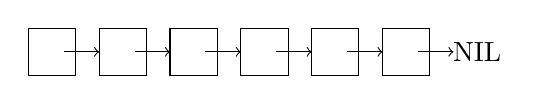
\begin{tikzpicture}[scale=3]
    \foreach \x in {-2, -1.7, ..., -0.4} {
      \draw (\x cm, 1cm) +(-0.1, -0.1) rectangle ++(0.1, 0.1);
      \draw[->] (\x cm, 1cm) +(0.05, 0) -- +(0.2, 0);
    }
    \draw (-0.2cm, 1cm) node {NIL};
    \end{tikzpicture}
  \caption{A list of nodes}
  \label{fig:list-example}
\end{figure}

Every node links to the next or NIL. We often define list with the compound structure\footnote{In most cases, the data stored in list have the same type. However, there is also heterogeneous list, like the list in Lisp for example.}, for example:

\lstset{frame=single}
\begin{lstlisting}[language=Bourbaki]
data List<A> {
    A key
    List<A> next
}
\end{lstlisting}

\index{List!empty} \index{List!empty testing}
Many traditional environments support the NIL concept. There are two ways to represent the empty list: one is to use NIL (or null, or $\nil$) directly; the other is to create a list, but put nothing as $[\ ]$. From implementation perspective, NIL need not allocate any memories, while $[\ ]$ does.

\subsection{Access}
\index{List!head} \index{List!tail} \index{List!Construction} \index{List!cons}
Given a none empty list $X$, define two functions\footnote{We often write function $f(x)$ as $f\ x$, and $f(x, y, ..., z)$ as $f\ x\ y\ ...\ z$.} to access the first element, and the rest sub-list. They are often called as \textit{first}\ $X$ and \textit{rest}\ $X$, or $head\ X$ and $tail\ X$\footnote{They are named as \texttt{car} and \texttt{cdr} in Lisp due to the design of machine registers\cite{SICP}.}. Conversely, we can construct a list from an element $x$ and another list $xs$ (can be empty), as $x \cons xs$. It is called the \texttt{cons} operation. We have the following equations:

\be
\begin{cases}
head\ (x \cons xs) & = x \\
tail\ (x \cons xs) & = xs
\end{cases}
\label{eq:list-head-tail}
\ee

For a none empty list $X$, we also denote the first element as $x_1$, and the rest sub-list as $X'$. For example, when $X = [x_1, x_2, x_3, ...]$, then $X' = [x_2, x_3, ...]$.

\begin{Exercise}
\Question{For list of type $A$, suppose we can test if any two elements $x, y \in A$ are equal, define an algorithm to test if two lists are identical.}
\end{Exercise}

\section{Basic operations}
\index{List!length}
From the definition, we can count the length recursively. the length of the empty list is 0, or it is 1 plus the length of the sub-list.

\be
\begin{array}{rcl}
length\ [\ ] & = & 0 \\
length\ (x \cons xs) & = & 1 + length\ xs
\end{array}
\ee

We traverse the list to count the length, the performance is bound to $O(n)$, where $n$ is the number of elements. We use $|X|$ as the length of $X$ when the context is clear. To avoid repeatedly counting, we can persist the length in a variable, and update it when mutate (add or delete). Below is the iterative length counting:

\begin{algorithmic}[1]
\Function{Length}{X}
  \State $n \gets 0$
  \While{$X \neq $ NIL}
    \State $n \gets n + 1$
    \State $X \gets $ \Call{Next}{$X$}
  \EndWhile
  \State \Return $n$
\EndFunction
\end{algorithmic}

\subsection{index}
\index{List!index} \index{List!get at}
Array supports random access at position $i$ in constant time, while we need traverse the list $i$ steps to access the target element.

\be
getAt\ i\ (x \cons xs) = \begin{cases}
  i = 0: & x \\
  i \neq 0: & getAt\ (i - 1)\ xs \\
\end{cases}
\ee

We leave the empty list not handled. The behavior when $[\ ]$ is undefined. As such, the out of bound case also leads to the undefined behavior. If $i > |X|$, we end up the edge case to access the $(i-|X|)$ position of the empty list. On the other hand, if $i < 0$, after minus it by one, it's even farther away from 0, and finally ends up with some negative position of the empty list. $getAt$ is bound to $O(i)$ time as it advances the list $i$ steps. Below is the imperative implementation:

\begin{algorithmic}[1]
\Function{Get-At}{$i, X$}
  \While{$i \neq 0$}
    \State $X \gets $ \Call{Next}{$X$}  \Comment{error when $X$ = NIL}
    \State $i \gets i - 1$
  \EndWhile
  \State \Return \Call{First}{$X$}
\EndFunction
\end{algorithmic}

\begin{Exercise}
\Question{In the iterative \textproc{Get-At}($i, X$) implementation, what is the behavior when $X$ is empty? what if $i$ is out of the bound or negative?}
\end{Exercise}

\subsection{Last}
\index{List!last} \index{List!init}

There is a pair of symmetric operations to `first/rest', namely `last/init'. For a none empty list $X = [x_1, x_2, ..., x_n]$, function $last$ returns the tail element $x_n$, while $init$ returns the sub-list of $[x_1, x_2, ..., x_{n-1}]$. Although they are symmetric pairs left to right, `last/init' need traverse the list, hence are linear time.

\be
\begin{array}{cc}
  \begin{array}{rcl}
  last\ [x] & = & x \\
  last\ (x \cons xs) & = & last\ xs \\
  \end{array}
&
  \begin{array}{rcl}
  init\ [x] & = & [\ ] \\
  init\ (x:xs) & = & x : init\ xs \\
  \end{array}
\end{array}
\label{eq:list-last}
\ee

Both do not handle the empty list. The behavior is undefined with $[\ ]$. Below are the iterative implementation:

\begin{algorithmic}[1]
\Function{Last}{$X$}
  \State $x \gets $ NIL
  \While{$X \neq$ NIL}
    \State $x \gets $ \Call{First}{$X$}
    \State $X \gets $ \Call{Rest}{$X$}
  \EndWhile
  \State \Return $x$
\EndFunction
\Statex
\Function{Init}{$X$}
  \State $X' \gets $ NIL
  \While{\Call{Rest}{$X$} $\neq$ NIL} \Comment{Error when $X$ is NIL}
    \State $X' \gets$ \textproc{Cons}(\Call{First}{$X$}, $X'$)
    \State $X \gets $ \Call{Rest}{$X$}
  \EndWhile
  \State \Return \Call{Reverse}{$X'$}
\EndFunction
\end{algorithmic}

\textproc{Init} accumulates the result through \textproc{Cons}. However, the order is reversed. We need reverse (section \ref{sec:reverse}) it back.

\subsection{Right index}
\index{List!Right index} \index{List!rindex}

$last$ is a special case of right index. The generic case is to find the last $i$-th element (from right). The naive implementation traverses two rounds: count the length $n$ first, then access the $(n - i - 1)$-th element from left:

\[
  lastAt\ i\ X = getAt\ (|X| - i - 1)\ L
\]

The better solution uses two pointers $p_1, p_2$ with the distance if $i$, i.e., $rest^i(p_2) = p_1$, where $rest^i(p_2)$ means repeatedly apply $rest$ for $i$ times. When advance $p_2$ by $i$ steps, it meets $p_1$. $p_2$ starts from the head. Advance both pointers in parallel till $p_1$ arrives at tail. At this time point, $p_2$ exactly points to the $i$-th element from right. as shown in figure \ref{fig:list-rindex}. $p_1$ and $p_2$ form a sliding window of width $i$.

\begin{figure}[htbp]
  \centering
  \subcaptionbox{$p_2$ starts from the head, behind $p_1$ in $i$ steps.}{\includegraphics[scale=0.8]{img/list-rindex}} \\
  \subcaptionbox{When $p_1$ reaches the tail, $p_2$ points to the $i$-th element from right.}{\includegraphics[scale=0.8]{img/list-rindex-2}}
  \caption{Sliding window}
  \label{fig:list-rindex}
\end{figure}

\begin{algorithmic}[1]
\Function{Last-At}{$i, X$}
  \State $p \gets X$
  \While{$i > 0$}
    \State $X \gets $ \Call{Rest}{$X$} \Comment{Error if out of bound}
    \State $i \gets i - 1$
  \EndWhile
  \While{\Call{Rest}{$X$} $\neq$ NIL}
    \State $X \gets$ \Call{Rest}{$X$}
    \State $p \gets$ \Call{Rest}{$p$}
  \EndWhile
  \State \Return \Call{First}{$p$}
\EndFunction
\end{algorithmic}

We can't alter the pointers in purely functional settings. Instead, we advance two lists $X = [x_1, x_2, ..., x_n]$ and $Y = [x_i, x_{i+1}, ..., x_n]$ simultaneously, where $Y$ is the sub-list without the first $i - 1$ elements.

\be
lastAt\ i\ X\ = slide\ X\ (drop\ i\ X)
\ee

Where:

\be
\begin{array}{rcl}
slide\ (x \cons xs)\ [y] & = & x \\
slide\ (x \cons xs)\ (y \cons ys) & = & slide\ xs\ ys \\
\end{array}
\ee

Function $drop\ m\ X$ discards the first $m$ elements.

\be
\begin{array}{rcl}
drop\ 0\ xs & = & xs \\
drop\ m\ [\ ] & = & [\ ] \\
drop\ m\ (x \cons xs) & = & drop\ (m - 1)\ xs \\
\end{array}
\ee

\begin{Exercise}
\Question{In the \textproc{Init} algorithm, can we use \textproc{Append}($X'$, \textproc{First}($X$)) instead of \textproc{Cons}?}
\Question{How to handle empty list or out of bound error in \textproc{Last-At}?}
\end{Exercise}

\subsection{Mutate}
\index{List!mutate}
Mutate includes append, insert, update, and delete. The functional environment actually implements mutate by creating a new list for the changed part, while keeps (persists) the original one for reuse, or release at sometime (chapter 2 in \cite{okasaki-book}).

\index{List!append}
Append is the symmetric operation of $cons$, it appends element to the tail, while $cons$ add from head. It is also known as `snoc' (reverse of `cons'). As it need traverse the list to the tail, the performance is $O(n)$, where $n$ is the length. To avoid repeatedly traverse, we can persist the tail reference, and update it for changes.

\be
\begin{array}{rcl}
append\ [\ ]\  x & = & [x] \\
append\ (y \cons ys)\ x & = & y : append\ ys\ x \\
\end{array}
\ee

Below is the corresponding iterative implementation\footnote{The parameter orders are also symmetric: $cons\ x\ xs$ and $append\ xs\ x$}:

\begin{algorithmic}[1]
\Function{Append}{$X, x$}
  \If{$X = $ NIL}
    \State \Return \Call{Cons}{$x$, NIL}
  \EndIf
  \State $H \gets X$ \Comment{Copy of the head}
  \While{\Call{Rest}{$X$} $\neq$ NIL}
    \State $X \gets$ \Call{Rest}{$X$}
  \EndWhile
  \State \Call{Rest}{$X$} $\gets$ \Call{Cons}{$x$, NIL}
  \State \Return $H$
\EndFunction
\end{algorithmic}

To update the \textproc{Rest}, it is typically implemented by updating the \texttt{next} reference, for example:

\begin{lstlisting}[language=Bourbaki]
List<A> append(List<A> xs, A x) {
    if xs == null then return cons(x, null)
    var head = xs
    while xs.next != null {
        xs = xs.next
    }
    xs.next = cons(x, null)
    return head
}
\end{lstlisting}

\index{List!set at}
Similar to $getAt$, we need advance to the target position and change the element.

\be
\begin{array}{rcl}
setAt\ 0\ x\ (y \cons ys) & = & x : ys \\
setAt\ i\ x\ (y \cons ys) & = & y : setAt\ (i - 1)\ x\ ys \\
\end{array}
\ee

The $setAt$ is bound to $O(i)$ time, where $i$ is the position for update.

\begin{Exercise}
\Question{Add the `tail' reference, optimize the $append$ to constant time.}
\Question{When need update the tail reference? How does it affect the performance?}
\Question{Handle the empty list and out of bound error for $setAt$.}
\end{Exercise}

\subsubsection{insert}
\index{List!insert} \index{List!insert at}
There are two different cases about insertion: (1) insert an element at a given position: $insert\ i\ x\ X$, similar to $setAt$; (2) insert an element to a sorted list, and maintain the ordering.

\be
\begin{array}{rcl}
insert\ 0\ x\ ys & = & x : ys \\
insert\ i\ x\ (y \cons ys) & = & y : insert\ (i - 1)\ x\ ys \\
\end{array}
\ee

When $i$ exceeds the length, treat it as append (the exercise of this section). Below is the iterative implementation:

\begin{algorithmic}[1]
\Function{Insert}{$i, x, X$}
  \If{$i = 0$}
    \State \Return \Call{Cons}{$x, X$}
  \EndIf
  \State $H \gets X$
  \State $p \gets X$
  \While{$i > 0$ and $X \neq$ NIL}
    \State $p \gets X$
    \State $X \gets $ \Call{Rest}{$X$}
    \State $i \gets i - 1$
  \EndWhile
  \State \Call{Rest}{$p$} $\gets$ \Call{Cons}{$x, X$}
  \State \Return $H$
\EndFunction
\end{algorithmic}

Let the list $L = [x_1, x_2, ..., x_n]$ be sorted, i.e., for any position $1 \leq i \leq j \leq n$, then $x_i \leq x_j$. Where $\leq$ is abstract ordering. It can be $\geq$, subset between sets, and etc. We define $insert$ to maintain the ordering.

\be
\begin{array}{rcl}
insert\ x\ [\ ] & = & [x] \\
insert\ x\ (y \cons ys) & = & \begin{cases}
  x \leq y : & x \cons y \cons ys \\
  \text{否则} : & y : insert\ x\ ys \\
  \end{cases}
\end{array}
\label{eq:list-ordered-insert}
\ee

Since it need compare elements one by one, the performance is bound to $O(n)$ time, where $n$ is the length. Below is the iterative implementation:

\begin{algorithmic}[1]
\Function{Insert}{$x, X$}
  \If{$X = $ NIL or $x <$ \Call{First}{$X$}}
    \State \Return \Call{Cons}{$x, X$}
  \EndIf
  \State $H \gets X$
  \While{\Call{Rest}{$X$} $\neq $ NIL and \textproc{First}(\Call{Rest}{$X$}) $< x$}
    \State $X \gets $ \Call{Rest}{$X$}
  \EndWhile
  \State \Call{Rest}{$X$} $\gets$ \textproc{Cons}($x$, \Call{Rest}{$X$})
  \State \Return $H$
\EndFunction
\end{algorithmic}

\label{sec:isort}
With $insert$, we can further define the insertion sort: repeatedly insert elements to the empty list. Since each insert takes liner time, the overall time is bound to $O(n^2)$.

\be
\begin{array}{rcl}
sort\ [\ ] & = & [\ ] \\
sort\ (x \cons xs) & = & insert\ x\ (sort\ xs) \\
\end{array}
\ee

We can eliminate the recursion to implement the iterative implementation. Scan the list, and insert elements one by one:

\begin{algorithmic}[1]
\Function{Sort}{$X$}
  \State $S \gets$ NIL
  \While{$X \neq$ NIL}
    \State $S \gets$ \textproc{Insert}(\Call{First}{$X$}, $S$)
    \State $X \gets$ \Call{Rest}{$X$}
  \EndWhile
  \State \Return $S$
\EndFunction
\end{algorithmic}

At any time during loop, the $S$ is sorted. The recursive implementation processes the list from right, while the iterative one is from left. We'll use `tail-recursion' in section \ref{sec:tail-call} to eliminate this difference. Chapter 3 is about insertion sort in detail, including performance analysis and optimization.

\begin{Exercise}
\Question{Handle the out-of-bound case when insert, treat it as append.}
\Question{Implement insert for array. When insert at position $i$, all elements after $i$ need shift to the end.}
\end{Exercise}

\subsubsection{delete}
\index{List!delete} \index{List!delete at}
Symmetric to insert, there are two cases for deletion: (1). delete the element at a position $delAt\ i\ X$; (2) look up then delete the element of a given value $delete\ x\ X$. To delete the element at position $i$, we advance $i$ steps to the target position, then by pass the element, and link the rest sub-list.

\be
\begin{array}{rcl}
delAt\ i\ [\ ] & = & [\ ] \\
delAt\ 0\ (x \cons xs) & = & xs \\
delAt\ i\ (x \cons xs) & = & x : delAt\ (i - 1)\ xs \\
\end{array}
\ee

It is bound to $O(i)$ time as we need advance $i$ steps to delete. Below is the iterative implementation.

\begin{algorithmic}[1]
\Function{Del-At}{$i, X$}
  \State $S \gets$ \Call{Cons}{$\perp, X$} \Comment{Sentinel node}
  \State $p \gets S$
  \While{$i > 0$ and $X \neq$ NIL}
    \State $i \gets i - 1$
    \State $p \gets X$
    \State $X \gets $ \Call{Rest}{$X$}
  \EndWhile
  \If{$X \neq$ NIL}
    \State \Call{Rest}{$p$} $\gets$ \Call{Rest}{$X$}
  \EndIf
  \State \Return \Call{Rest}{$S$}
\EndFunction
\end{algorithmic}

To simplify the implementation, we introduce a sentinel node $S$, it contains a special value $\perp$, and points to $X$. With $S$, we are save to cut-off any node in $X$ even for the head. Finally, we return the list after $S$ as the result, and discard $S$. For `find and delete', there are two sub-cases: (1) find and delete the first occurrence of a value; (2) remove all the occurrences. The later is more generic (see the exercise).

\be
\begin{array}{rcl}
delete\ x\ [\ ] & = & [\ ] \\
delete\ x\ (y \cons ys) & = & \begin{cases}
  x = y : & ys \\
  x \neq y : & y : delete\ x\  ys \\
  \end{cases} \\
\end{array}
\label{eq:list-delete}
\ee

Because we scan the lit to find the target element, the time is bound to $O(n)$, where $n$ is the length. We use a sentinel node to simplify the iterative implementation too:

\begin{algorithmic}[1]
\Function{Delete}{$x, X$}
  \State $S \gets$ \Call{Cons}{$\perp, X$}
  \State $p \gets X$
  \While{$X \neq$ NIL and \Call{First}{$X$} $\neq x$}
    \State $p \gets X$
    \State $X \gets$ \Call{Rest}{$X$}
  \EndWhile
  \If{$X \neq$ NIL}
    \State \Call{Rest}{$p$} $\gets$ \Call{Rest}{$X$}
  \EndIf
  \State \Return \Call{Rest}{$S$}
\EndFunction
\end{algorithmic}

\begin{Exercise}
\Question{Implement the algorithm to find and delete all occurrences of a given value.}
\Question{Design the delete algorithm for array, all elements after the delete position need shift to front.}
\end{Exercise}

\subsubsection{concatenate}
\label{concat} \index{List!concat}

Append is a special case for concatenation. It adds only one element, while concatenation adds multiple. However, the performance would be quadratic if repeatedly append. Let $|xs| = n$, $|ys| = m$ be the lengths, we need advance to the tail of $xs$ for $m$ times, the performance is $O(n + (n + 1) + ... + (n + m)) = O(nm + m^2)$.

\[
\begin{array}{rcl}
xs \doubleplus [\ ] & = & xs \\
xs \doubleplus (y \cons ys) & = & append\ xs\ y \doubleplus ys \\
\end{array}
\]

While the `cons' is fast (constant time), we can traverse to the tail of $xs$ only once, then link to $ys$.

\be
\begin{array}{rcl}
[\ ] \doubleplus ys & = & ys \\
xs \doubleplus [\ ] & = & xs \\
(x \cons xs) \doubleplus ys & = & x : (xs \doubleplus ys) \\
\end{array}
\ee

This improvement has the performance of $O(n)$. In imperative settings, we can implement concatenation in constant time with the tail reference variable (see exercise).

\begin{algorithmic}[1]
\Function{Concat}{$X, Y$}
  \If{$X = $ NIL}
    \State \Return $Y$
  \EndIf
  \If{$Y = $ NIL}
    \State \Return $X$
  \EndIf
  \State $H \gets X$
  \While{\Call{Rest}{$X$} $\neq$ NIL}
    \State $X \gets$ \Call{Rest}{$X$}
  \EndWhile
  \State \Call{Rest}{$X$} $\gets Y$
  \State \Return $H$
\EndFunction
\end{algorithmic}

\subsection{sum and product}
\index{List!sum} \index{List!product}
We often need to calculate the sum or product of a list. They have the same structure. We will introduce how to abstract them to higher order computation in section \ref{sec:fold}. For empty list, define the sum as 0, the product as 1.

\be
\begin{array}{cc}
  \begin{array}{rcl}
  sum\ [\ ] & = & 0 \\
  sum\ (x \cons xs) & = & x + sum\ xs \\
  \end{array}
  &
  \begin{array}{rcl}
  product\ [\ ] & = & 1 \\
  product (x \cons xs) & = & x \cdot product\ xs \\
  \end{array}
\end{array}
\ee

\index{Tail call} \index{Tail recursion} \index{Tail recursive call}
\label{sec:tail-call}

Both need traverse the list, hence the performance is $O(n)$, where $n$ is the length. They compute from right to left. We can change to {\em accumulate} the result from left. For sum, accumulate from 0; while for product, accumulate from 1.

\be
\begin{array}{cc}
  \begin{array}{rcl}
  sum'\ a\ [\ ] & = & a \\
  sum'\ a\ (x \cons xs) & = & sum\ (x + a)\ xs \\
  \end{array}
  &
  \begin{array}{rcl}
  prod'\ a\ [\ ] & = & a \\
  prod'\ a\ (x \cons xs) & = & prod'\ (x \cdot a)\ xs \\
  \end{array} \\
\end{array}
\ee

Given a list, we call $sum'$ with 0, and $prod'$ with 1 as the accumulators:

\be
sum\ xs = sum'\ 0\ xs
\quad \quad \quad
product\ xs = prod'\ 1\ xs
\ee

Or in Curried form:

\[
sum = sum'\ 0 \quad \quad \quad product = prod'\ 1
\]

\index{Curried Form} \index{Currying}
Curried form was introduced by Schönfinkel (1889 - 1942) in 1924, then widely used by Haskell Curry from 1958. It is known as {\em Currying}\cite{slpj-book-1987}. For a function taking 2 parameters $f(x, y)$, when fix $x$ with a value, it becomes a function of $y$: $g(y) = f(x, y)$ or $g = f\ x$. For multiple variables of $f(x, y, ..., z)$, we convert it to a series of Curried functions: $f, f\ x, f\ x\ y, ...$, each takes one parameter: $f(x, y, ..., z) = f(x)(y)...(z) = f\ x\ y\ ...\ z$.

The accumulated implementation computes from left to right, needn't book keeping any context, state, or intermediate result for recursion. All states are either passed as argument (for example $a$), or dropped (for example the previous element). We can further optimize such recursive calls to loops. Because the recursion happens at the tail of the function, we call them {\em tail recursion} (or `tail call'), and the process to eliminate recursion as `tail recursion optimization'\cite{wiki-tail-call}. It greatly improves the performance and avoid stack overflow due to deep recursions. In section \ref{sec:isort} about insertion sort, the recursive implementation sorts elements form right. We also optimize it to tail call:

\be
\begin{array}{rcl}
sort'\ a\ [\ ] & = & a \\
sort'\ a\ (x \cons xs) & = & sort'\ (insert\ x\ a)\ xs \\
\end{array}
\ee

We pass $[\ ]$ to start sorting (Curried form): $sort = sort'\ [\ ]$. As a typical tail call example, consider how to compute $b^n$ effectively? (problem 1.16 in \cite{SICP}.) A direct implementation repeatedly multiplies $b$ for $n$ times from 1, which is bound to $O(n)$ time:

\begin{algorithmic}[1]
\Function{Pow}{$b, n$}
  \State $x \gets 1$
  \Loop{ $n$ times}
    \State $x \gets x \cdot b$
  \EndLoop
  \State \Return $x$
\EndFunction
\end{algorithmic}

When compute $b^8$, after the first 2 loops, we get $x = b^2$. At this stage, we needn't multiply $x$ with $b$ to get $b^3$, but directly compute $x^2$, which gives $b^4$. If do this again, we get $(b^4)^2 = b^8$. We only need loop 3 times, but not 8 times. If $n = 2^m$ for some none negative integer $m$, we can compute $b^n$ fast as below:

\[
\begin{array}{rcl}
b^1 & = & b \\
b^n & = & (b^{\frac{n}{2}})^2 \\
\end{array}
\]

We next extend this divide and conquer method to any none negative integer $n$: if $n = 0$, define $b^0 = 1$; if $n$ is even, we halve $n$, to compute $b^{\frac{n}{2}}$. Then square it; if $n$ is odd, since $n-1$ is even, we recursively compute $b^{n-1}$, then multiply $b$ atop it.

\be
\begin{array}{rcl}
b^0 & = & 1 \\
b^n & = & \begin{cases}
2 | n : & (b^{\frac{n}{2}})^2 \\
\text{otherwise}: & b \cdot b^{n-1} \\
\end{cases}
\end{array}
\ee

However, the 2nd clause blocks us from turning it to tail recursive. Alternatively, we square the base number, and halve the exponent.

\be
\begin{array}{rcl}
b^0 & = & 1 \\
b^n & = & \begin{cases}
2 | n : & (b^2)^{\frac{n}{2}} \\
\text{otherwise}: & b \cdot b^{n-1} \\
\end{cases}
\end{array}
\ee

With this change, we get a tail recursive function to compute $b^n = pow(b, n, 1)$.

\be
\begin{array}{rcl}
pow(b, 0, a) & = & a \\
pow(b, n, a) & = & \begin{cases}
  2 | n : & pow(b^2, \dfrac{n}{2}, a) \\
  \text{otherwise}: & pow(b, n - 1, ab) \\
\end{cases}
\end{array}
\ee

This implementation is bound to $O(\lg n)$ time. We can improve it further. Represent $n$ in binary format $n = (a_ma_{m-1}...a_1a_0)_2$. We need compute $b^{2^i}$ if $a_i = 1$, similar to the Binomial heap (\autoref{sec:binomial-heap}, chapter 10) algorithm. Finally, we multiplying them together. For example, when compute $b^{11}$, as $11 = (1011)_2 = 2^3 + 2 +1$, gives $b^{11} = b^{2^3} \times b^2 \times b$. We follow these steps:

\begin{enumerate}
\item compute $b^1$, which is $b$;
\item Square to $b^2$;
\item Square to $b^{2^2}$;
\item Square to $b^{2^3}$.
\end{enumerate}

Finally, multiply the result of step 1, 2, and 4 to get $b^{11}$.

\be
\begin{array}{rcl}
pow(b, 0, a) & = & a \\
pow(b, n, a) & = & \begin{cases}
  2 | n : & pow(b^2, \dfrac{n}{2}, a) \\
  \text{otherwise}: & pow(b^2, \lfloor \dfrac{n}{2} \rfloor, ab) \\
  \end{cases}
\end{array}
\ee

This algorithm essentially shifts $n$ to right 1 bit a time (divide $n$ by 2). If the LSB (the least significant bit) is 0, $n$ is even, squares the base and keeps the accumulator $a$ unchanged. If the LSB is 1, $n$ is odd, squares the base and accumulates it to $a$. When $n$ is zero, we exhaust all bits, $a$ is the final result. At any time, the updated base $b'$, the shifted exponent $n'$, and the accumulator $a$ satisfy the invariant $b^n = a (b')^{n'}$.The previous implementation minus one for odd $n$, the improvement halves $n$ every time. It exactly runs $m$ rounds, where $m$ is the number of bits. We leave the imperative implementation as exercise.

Back to the sum and product, the iterative implementation applies plus and multiply while traversing:

\begin{algorithmic}[1]
\Function{Sum}{$X$}
  \State $s \gets 0$
  \While{$X \neq$ NIL}
    \State $s \gets s +$ \Call{First}{$X$}
    \State $X \gets$ \Call{Rest}{$X$}
  \EndWhile
  \State \Return $s$
\EndFunction
\Statex
\Function{Product}{$X$}
  \State $p \gets 1$
  \While{$X \neq$ NIL}
    \State $p \gets p\ \cdot$ \Call{First}{$X$}
    \State $X \gets$ \Call{Rest}{$X$}
  \EndWhile
  \State \Return $p$
\EndFunction
\end{algorithmic}

With product, we can define factorial of $n$ as: $n! = product\ [1..n]$.

\subsection{maximum and minimum}
\index{List!maximum} \index{List!minimum}

For a list of comparable elements (we can define order for any two elements), there is the maximum and minimum. $max/min$ share the same structure:

\be
\resizebox{\linewidth}{!}{\ensuremath{
\begin{array}{cc}
  \begin{array}{rcl}
  \min\ [x] & = & x \\
  \min\ (x \cons xs) & = & \begin{cases}
    x < \min\ xs : & x \\
    \text{otherwise}: & \min\ xs \\
  \end{cases}
  \end{array}
&
  \begin{array}{rcl}
  \max\ [x] & = & x \\
  \max\ (x \cons xs) & = & \begin{cases}
    x > \max\ xs : & x \\
    \text{otherwise}: & \max\ xs \\
  \end{cases}
  \end{array}
\end{array}
}}
\ee

Both process the list from right. We can change them to tail recursive. It also makes the computation `on-line', that at any time, the accumulator is the min/max so far. Use $min$ for example:

\be
\begin{array}{rcl}
\min'\ a\ [\ ] & = & a \\
\min'\ a\ (x \cons xs) & = & \begin{cases}
  x < a : & \min'\ x\ xs \\
  \text{否则} : & \min'\ a\ xs \\
  \end{cases}
\end{array}
\ee

Different from $sum'/prod'$, we can't pass a fixed starting value to $min'/max'$, unless $\pm \infty$ (Curried form):

\[
  \textstyle \min = \min'\ \infty \quad \quad \quad \max = \max'\ -\infty
\]

We can pass the first element given min/max only takes none empty list:

\be
  \textstyle
  \min\ (x \cons xs) = \min'\ x\ xs
  \quad \quad \quad
  \max\ (x \cons xs) = \max'\ x\ xs
\ee

We can optimize the tail recursive implementation with loops. Use the \textproc{Min} for example.

\begin{algorithmic}[1]
\Function{Min}{$X$}
  \State $m \gets$ \Call{First}{$X$}
  \State $X \gets$ \Call{Rest}{$X$}
  \While{$X \neq$ NIL}
    \If{\Call{First}{$X$} $< m$ }
      \State $m \gets$ \Call{First}{$X$}
    \EndIf
    \State $X \gets$ \Call{Rest}{$X$}
  \EndWhile
  \State \Return $m$
\EndFunction
\end{algorithmic}

Alternatively, we can re-use the first element as the accumulator. Every time, we compare the first two elements, and drop one. Below is the example for $min$. $max$ is symmetric.

\be
\begin{array}{rcl}
\min\ [x] & = & x \\
\min\ (x_1 \cons x_2 \cons xs) & = & \begin{cases}
  x_1 < x_2 : & \min\ (x_1 \cons xs) \\
  \text{otherwise}: & \min\ (x_2 \cons xs) \\
  \end{cases}
\end{array}
\ee

\begin{Exercise}
\Question{Change $length$ to tail recursive.}
\Question{Change the insertion sort to tail recursive.}
\Question{Compute $b^n$ through the binary format of $n$.}
\end{Exercise}

\section{Transform}
\index{List!Transform}

In algebra, there are two types of transformation: one keeps the list structure, but only transforms the elements; the other alter the list structure, hence the result is not isomorphic. Particularly, we call the former {\em map}.

\subsection{map and for-each}
\index{List!map}

The first example converts a list of numbers to strings. Transform [3, 1, 2, 4, 5] to [``three'', ``one'', ``two'', ``four'', ``five'']

\be
\begin{array}{rcl}
toStr\ [\ ] & = & [\ ] \\
toStr\ (x \cons xs) & = & (str\ x) : toStr\ xs \\
\end{array}
\label{eq:tostr}
\ee

For the second example, given a dictionary, which is a list of words grouped by their initials:

\begin{Verbatim}[fontsize=\footnotesize]
[[a, an, another, ... ],
 [bat, bath, bool, bus, ...],
 ...,
 [zero, zoo, ...]]
\end{Verbatim}

Next process a text ({\em Hamlet} for example), augment each word with the number of occurrence, like:

\begin{Verbatim}[fontsize=\footnotesize]
[[(a, 1041), (an, 432), (another, 802), ... ],
 [(bat, 5), (bath, 34), (bool, 11), (bus, 0), ...],
 ...,
 [(zero 12), (zoo, 0), ...]]
\end{Verbatim}

Now for every initial letter, which word does occur most? The answer is a list of words, that every one has the most occurrences in the group, like \texttt{[a, but, can, ...]}. We need a program that transforms \textbf{a list of groups of word-number pairs} into \textbf{a list of words}. First, define a function, which takes a list of word-number pairs, finds the word paired with the biggest number. Sort is overkill. We need a special max function $maxBy\ cmp\ xs$, where $cmp$ is the generic compare function.

\be
\begin{array}{rcl}
maxBy\ cmp\ [x] & = & x \\
maxBy\ cmp\ (x_1 \cons x_2 \cons xs) & = & \begin{cases}
  cmp\ x_1\ x_2 : & maxBy\ cmp\ (x_2 \cons xs) \\
  \text{otherwise} : & maxBy\ cmp\ (x_1 \cons xs) \\
  \end{cases}
\end{array}
\ee

For a pair $p = (a, b)$ we define two functions:

\be
\begin{cases}
fst\ (a, b) = & a \\
snd\ (a, b) = & b \\
\end{cases}
\ee

Then define a special compare function for word-count pairs:

\be
less\ p_1\ p_2 = snd\ p_1 < snd\ p_2
\ee

Then pass $less$ to $maxBy$ (in Curried form): $\max'' = maxBy\ less$. Finally, call $max''$ to process the list:

\be
\begin{array}{rcl}
solve\ [\ ] & = & [\ ] \\
solve\ (x \cons xs) & = & (fst\ (\max''\ x)) : solve\ xs \\
\end{array}
\label{eq:solve}
\ee

\index{List!map}

$solve$ and $toStr$ share the same structure for different problems. We abstract this common structure as {\em map}:

\be
\begin{array}{rcl}
map\ f\ [\ ] & = & [\ ] \\
map\ f\ (x \cons xs) & = & (f\ x) : map\ f\ xs \\
\end{array}
\ee

$map$ takes a function $f$, applies it to every element to form a new list. A function that computes with other functions is called {\em high-order} function. Let the type of $f$ is $A \to B$. It sends an element of $A$ to the result of $B$, the type of map is:

\be
map :: (A \to B) \to [A] \to [B]
\ee

Read as: map takes a function of $A \to B$, converts a list $[A]$ to another list $[B]$. We can define the above two examples with map as below (in Curried form):

\[
\textstyle
toStr = map\ str \quad \quad \quad
solve = map\ (fst \circ \max'')
\]

Where $f \circ g$ is function composition, i.e. first apply $g$ then apply $f$. $(f \circ g)\ x = f(g(x))$, read as $f$ after $g$. From the set theory point of view. Function $y = f(x)$ defines the map from $x$ in set $X$ to $y$ in set $Y$:

\be
Y = \{ f(x) | x \in X \}
\ee

\index{List!ZF expression} \index{List!list comprehension}
This type of set definition is called Zermelo-Frankel set abstraction (known as ZF expression) \cite{algo-fp}. The difference is that the mapping is from a list (but not set) to another: $Y = [f(x) | x \gets Y]$. There can be duplicated elements. For list, such ZF style expression is called {\em list comprehension}. It is a powerful tool. let us see how to realize the permutation algorithm for example. Extend from full-permutations\cite{algo-fp}\cite{erlang}, we define a generic $perm\ X\ r$, that permutes $r$ out of the total $n$ elements in list $X$. There are total $P_n^r = \dfrac{n!}{(n-r)!}$ permutations.

\be
\resizebox{\linewidth}{!}{\ensuremath{
perm\ X\ r = \begin{cases}
  |X| < r\ \text{or}\ r = 0: & [[\ ]] \\
  \text{otherwise}: & [ x\cons ys \ |\ x \gets X, ys \gets perm\ (delete\ x\ X)\ (r - 1)] \\
  \end{cases}
}}
\ee

If pick zero element, or there are too few (less than $r$), the result is a list of empty[[\ ]]; otherwise, for every $x$ in $X$, we recursively pick $r-1$ out of the rest $n-1$ elements; then prepend $x$ for each.

We use a sentinel node in the iterative \textproc{Map} implementation.

\begin{algorithmic}[1]
\Function{Map}{$f, X$}
  \State $X' \gets$ \Call{Cons}{$\perp$, NIL} \Comment{the sentinel}
  \State $p \gets X'$
  \While{$X \neq$ NIL}
    \State $x \gets$ \Call{First}{$X$}
    \State $X \gets$ \Call{Rest}{$X$}
    \State \Call{Rest}{$p$} $\gets$ \Call{Cons}{$f(x)$, NIL}
    \State $p \gets$ \Call{Rest}{$p$}
  \EndWhile
  \State \Return \Call{Rest}{$X'$} \Comment{discard the sentinel}
\EndFunction
\end{algorithmic}

\subsubsection{For each}
\index{List!for each}

Sometimes we only need process the elements one by one without building the new list, for example, print every element:

\begin{algorithmic}[1]
\Function{Print}{$X$}
  \While{$X \neq$ NIL}
    \State print \Call{First}{$X$}
    \State $X \gets$ \Call{Rest}{$X$}
  \EndWhile
\EndFunction
\end{algorithmic}

More generally, we pass a procedure $P$, then apply $P$ to each element.

\begin{algorithmic}[1]
\Function{For-Each}{$P, X$}
  \While{$X \neq$ NIL}
    \State \textproc{P}(\Call{First}{$X$})
    \State $X \gets$ \Call{Rest}{$X$}
  \EndWhile
\EndFunction
\end{algorithmic}

For example, let us solve the ``$n$-lights puzzle''\cite{poj-drunk-jailer} with map. There are $n$ lights in a room, all are off. We execute the following $n$ rounds:

\begin{enumerate}
\item Switch all lights on;
\item Switch lights of number 2, 4, 6, ... , that every other light is switched;
\item Switch every third lights, number 3, 6, 9, ... ;
\item ...
\end{enumerate}

At the last round, only the $n$-th light is switched. How many lights are on in the end? We start with a brute-force solution. Represent the $n$ lights as a list of 0/1 numbers (0: off, 1: on). Start from all zeros: [0, 0, ..., 0]. Label the light from 1 to $n$, then map them to ($i$, on/off) pairs:

\[
lights = map\ (i \mapsto (i, 0))\ [1, 2, ..., n]
\]

It binds each number to zero, i.e., a list of pairs: $L$ = [(1, 0), (2, 0), ..., (n, 0)]. We operate this list of pairs $n$ rounds. In the $i$-th round, for every pair $(j, x)$, if $i | j$ (meaning $j \bmod i = 0$), then switch it on/off. As $1 - 0 = 1$ and $1 - 1 = 0$, we switch $x$ to $1 - x$.

\be
switch\ i\ (j, x)) = \begin{cases}
  j \bmod i = 0 : & (j, 1 - x) \\
  \text{否则}: & (j, x) \\
  \end{cases}
\ee

Realize the $i$-th round of operation as $map\ (switch\ i)\ L$ (we use the Curried form of $switch$). Next, define a function $op()$, which performs mapping on $L$ over and over for $n$ rounds: $op\ [1, 2, ..., n]\ L$.

\be
\begin{array}{rcl}
op\ [\ ]\ L & = & L \\
op\ (i \cons is)\ L & = & op\ is\ (map\ (switch\ i)\ L) \\
\end{array}
\ee

Finally, sum the second value of each pair to get the answer.

\be
solve\ n = sum\ (map\ snd\ (op\ [1, 2, ..., n]\ L))
\ee

Below is the example Haskell implementation:

\begin{Haskell}
solve = sum . (map snd) . proc  where
    lights = map (\i -> (i, 0)) [1..n]
    proc n = operate [1..n] lights
    operate [] xs = xs
    operate (i:is) xs = operate is (map (switch i) xs)
    switch i (j, x) = if j `mod` i == 0 then (j, 1 - x) else (j, x)
\end{Haskell}

Run this program from 1 to 100 lights, below are the answers (added line breaks):

\begin{Verbatim}[fontsize=\footnotesize]
[1,1,1,
 2,2,2,2,2,
 3,3,3,3,3,3,3,
 4,4,4,4,4,4,4,4,4,
 5,5,5,5,5,5,5,5,5,5,5,
 6,6,6,6,6,6,6,6,6,6,6,6,6,
 7,7,7,7,7,7,7,7,7,7,7,7,7,7,7,
 8,8,8,8,8,8,8,8,8,8,8,8,8,8,8,8,8,
 9,9,9,9,9,9,9,9,9,9,9,9,9,9,9,9,9,9,9,10]
\end{Verbatim}

They form a pattern: the first 3 answers are 1; the 4-th to the 8-th answers are 2; the 9-th to the 15-th answers are 3; ... It seems that the $i^2$-th to the $((i+1)^2-1)$-th answers are $i$. Let's prove it:

\begin{proof}
Given $n$ lights labeled from 1 to $n$, all light are off when start. The lights which are switched odd times are on finally. For every light $i$, we switch it at round $j$ if $j$ divides $i$ ($j | i$). Only the lights which have odd number of factors are on in the end. The key point to solve this puzzle, is to find all the numbers that have odd number of factors. For any natural number $n$, let $S$ be the set of all factors of $n$. Initialize $S$ as $\varnothing$. If $p$ is a factor of $n$, there must exist a natural number $q$ such that $n = p q$. It means $q$ is also a factor of $n$. We add 2 different factors to set $S$ if and only if $p \neq q$, which keeps $|S|$ even all the time unless $p = q$. In such case, $n$ is a square number. We can only add 1 factor to set $S$, which leads to odd number of factors.
\end{proof}

We have a fast solution by counting the square numbers under $n$.

\be
solve(n) = \lfloor \sqrt{n} \rfloor
\ee

Below Haskell example program outputs the answer for 1, 2, ..., 100 lights:

\begin{Haskell}
map (floor . sqrt) [1..100]
\end{Haskell}

Map is abstract, does not limit to list, but applies to many complex algebraic structures. The next chapter explains how to map trees. We can apply mapping as long as we can traverse the structure, and the empty is defined.

\subsection{reverse}
\index{List!reverse} \label{sec:reverse}

It's a good exercise to reverse a singly linked-list with constant space. One must carefully manipulate the node reference, while there exists an easy method: (1) Write a purely recursive solution; (2) Change it to tail recursive; (3) Convert to imperative implementation. The purely recursive solution is direct:

\[
\begin{array}{rcl}
reverse [\ ] & = & [\ ] \\
reverse (x \cons xs) & = & append\ (reverse\ xs)\ x \\
\end{array}
\]

Next convert it to tail recursive. Use an accumulator to store the reversed part, start from an empty list: $reverse = reverse'\ [\ ]$

\be
\begin{array}{rcl}
reverse'\ a\ [\ ] & = & a \\
reverse'\ a\ (x \cons xs) & = & reverse'\ (x \cons a)\ xs \\
\end{array}
\ee

Different from appending, cons (:) takes constant time. We repeatedly extract the head element, and prepend to the accumulator. It likes to store the elements in a stack, then pop them out. The overall performance is $O(n)$, where $n$ is the length. Since tail call need not keep the context, we next convert it to iterative loops:

\begin{algorithmic}[1]
\Function{Reverse}{$X$}
  \State $A \gets$ NIL
  \While{$X \neq$ NIL}
    \State $A \gets $ \textproc{Cons}(\Call{First}{$X$}, $A$)
    \State $X \gets$ \Call{Rest}{$X$}
  \EndWhile
  \State \Return $A$
\EndFunction
\end{algorithmic}

However, this implementation creates a new reversed list, but not reverses in-place. We change it further:

\begin{lstlisting}[language=Bourbaki]
List<T> reverse(List<T> xs) {
  List<T> p, ys = null
  while xs != null {
    p = xs
    xs = xs.next
    p.next = ys
    ys = p
  }
  return ys
}
\end{lstlisting}

\begin{Exercise}
\Question{Given a number from 0 to 1 billion, write a program to `read' it out. for example, output string `one hundred and twenty three' for 123. What if there is decimal part?}
\Question{Find the maximum $v$ in a list of pairs $[(k, v)]$ in tail recursive way.}
\end{Exercise}

\section{Sub-list}
\index{List!Extract sub-list} \index{List!take} \index{List!drop} \index{List!split at}
One can slice an array fast, but need linear time to traverse and extract sub-list. $take$ extracts the first $n$ elements, it is equivalent get a sub-list from 1 to $n$: $sublist\ 1\ n\ X$. $drop$ discards the first $n$ elements. It is equivalent to get a sub-list from right: $sublist\ (n+1)\ |X|\ X$, which is symmetric to $take$:

\be
\resizebox{\linewidth}{!}{\ensuremath{
\begin{array}{cc}
  \begin{array}{rcl}
  take\ 0\ xs & = & [\ ] \\
  take\ n\ [\ ] & = & [\ ] \\
  take\ n\ (x \cons xs) & = & x : take\ (n - 1)\ xs \\
  \end{array}
&
  \begin{array}{rcl}
  drop\ 0\ xs & = & xs \\
  drop\ n\ [\ ] & = & [\ ] \\
  drop\ n\ (x \cons xs) & = & drop\ (n - 1)\ xs \\
  \end{array}
\end{array}
}}
\ee

When $n > |X|$ or $n < 0$, it ends up with the empty list case. We leave the imperative implementation as exercise. We can extract the sub-list at any position for a given length:

\be
sublist\ from\ cnt\ X = take\ cnt\ (drop\ (from - 1)\ X)
\ee

Or slice the list with left and right boundaries:

\be
slice\ from\ to\ X = drop\ (from - 1)\ (take\ to\ X)
\ee

\index{List!split at}
The range $[from, to]$ includes both ends. We can split the list at a position:

\be
splitAt\ i\ X = (take\ i\ X, drop\ i\ X)
\label{eq:split-at}
\ee

\begin{Exercise}
\Question{Define $sublist$ and $slice$ in Curried Form without $X$ as parameter.}
\end{Exercise}

\subsubsection{conditional take and drop}
\index{List!take while} \index{List!drop while}

We can extend $take/drop$ to keep taking or dropping as far as some condition is satisfied, Define \textit{takeWhile/dropWhile}, that scan every element with a predicate $p$, stop when any element doesn't satisfy. They ignore the rest even if some elements satisfy $p$. We'll see this different in the section of filtering.

\be
\resizebox{\linewidth}{!}{\ensuremath{
\begin{array}{cc}
  \begin{array}{rcl}
  \textit{takeWhile}\ p\ [\ ] & = & [\ ] \\
  \textit{takeWhile}\ p\ (x \cons xs) & = & \begin{cases}
    (p\ x) : & x : \textit{takeWhile}\ p\ xs \\
    \text{otherwise}: & [\ ] \\
    \end{cases}
  \end{array}
&
  \begin{array}{rcl}
  \textit{dropWhile}\ p\ [\ ] & = & [\ ] \\
  \textit{dropWhile}\ p\ (x \cons xs) & = & \begin{cases}
    (p\ x) : & \textit{dropWhile}\ p\ xs \\
    \text{otherwise}: & x \cons xs \\
    \end{cases}
  \end{array}
\end{array}
}}
\ee

\subsection{break and group}
Break and group are operations to re-arrange a list into multiple sub-lists. They typically perform the re-arrangement while traverse the list to keep the performance linear.

\subsubsection{break and span}
\index{List!break} \index{List!span}

$break/span$ can be considered as a general form of splitting. Instead of splitting at a given position, $break/span$ scans elements with a prediction. It extracts the longest prefix of the list against the condition, and returns it together with the rest as a pair.

There are two different cases. For a given predication, one is to pick the elements satisfied; the other is to pick the elements not satisfied. The former is called $span$, the later is called $break$.

\be
\begin{array}{rcl}
span(p,\ [\ ]) & = & ([\ ], [\ ]) \\
span(p,\ x:xs) & = & \begin{cases}
  p(x) : & (x : A,\ B)\ \text{where}\ (A, B) = span(p, xs) \\
  otherwise : & ([\ ],\ x:xs) \\
  \end{cases}
\end{array}
\label{eq:span}
\ee

and we can define $break$ with span by negating the predication in Curried form:

\be
break(p) = span(\lnot p)
\ee

Both $span$ and $break$ find the longest {\em prefix}. They stop immediately when the condition does not meet and ignores the rest. Below is the iterative implementation for span:

\begin{algorithmic}[1]
\Function{Span}{$p, L$}
  \State $A \gets $ NIL
  \While{$L \neq$ NIL and $p$(\Call{First}{$L$})}
    \State $A \gets $ \textproc{Cons}(\Call{First}{$L$}, $A$)
    \State $L \gets $ \Call{Rest}{$L$}
  \EndWhile
  \State \Return $(A, L)$
\EndFunction
\end{algorithmic}

This algorithm creates a new list to hold the longest prefix, another option is to reuse the original list and break it in-place:

\begin{algorithmic}[1]
\Function{Span}{$p, L$}
  \State $A \gets L$
  \State $tail \gets$ NIL
  \While{$L \neq$ NIL and $p$(\Call{First}{$L$})}
    \State $tail \gets L$
    \State $L \gets $ \Call{Rest}{$L$}
  \EndWhile
  \If{$tail =$ NIL}
    \State \Return (NIL, $L$)
  \EndIf
  \State \Call{Rest}{$tail$} $\gets$ NIL
  \State \Return $(A, L)$
\EndFunction
\end{algorithmic}

\subsubsection{group}
\index{List!group}
span breaks list into two parts, group divides list into multiple sub-lists. For example, we can use group to change a long word into small units, each contains consecutive same characters:

\begin{Haskell}
group ``Mississippi'' = [``M'', ``i'', ``ss'', ``i'',
                         ``ss'',``i'', ``pp'', ``i'']
\end{Haskell}

For another example, given a list of numbers:

\[
L = [15, 9, 0, 12, 11, 7, 10, 5, 6, 13, 1, 4, 8, 3, 14, 2]
\]

We can divide it into small lists, each one is in descending order:

\[
group(L) = [[15, 9, 0], [12, 11, 7], [10, 5], [6], [13, 1], [4], [8, 3], [14, 2]]
\]

These are useful operations. The string groups can be used to build Radix tree, a data structure support fast text search. The number groups can be used to implement nature merge sort algorithm. We'll introduce them in later chapters.

We can abstract the group condition as a relation $\sim$. It tests whether two consecutive elements $x$, $y$ are generic `equivalent': $x \sim y$. We scan and list and compare two elements each time. If they match, we add both to a group; otherwise, only add $x$ to the group, and use $y$ to initialize another group.

\be
\begin{array}{rcl}
group(\sim,\ [\ ]) & = & [[\ ]] \\
group(\sim,\ [x]) & = & [[x]] \\
group(\sim,\ x:y:xs) & = & \begin{cases}
  x \sim y : & (x:ys):yss \\
  otherwise: & [x]:ys:yss \\
\end{cases}
\end{array}
\ee

where $(ys:yss) = group(\sim, xs)$. This algorithm is bound to $O(n)$ time, where $n$ is the length. We can also implement the iterative group algorithm. For the none empty list $L$, we initialize the result groups as $[[x_1]]$, where $x_1$ is the first element. We scan the list from the second one, append it to the last group if the two consecutive elements are `equivalent'; otherwise we start a new group.

\begin{algorithmic}[1]
\Function{Group}{$\sim, L$}
  \If{$L = $ NIL}
    \State \Return [NIL]
  \EndIf
  \State $x \gets$ \Call{First}{$L$}
  \State $L \gets$ \Call{Rest}{$L$}
  \State $g \gets [x]$
  \State $G \gets [g]$
  \While{$L \neq$ NIL}
    \State $y \gets$ \Call{First}{$L$}
    \If{$x \sim y$}
      \State $g \gets $ \Call{Append}{$g, y$}
    \Else
      \State $g \gets [y]$
      \State $G \gets$ \Call{Append}{$G, g$}
    \EndIf
    \State $x \gets y$
    \State $L \gets$ \Call{Next}{$L$}
  \EndWhile
  \State \Return $G$
\EndFunction
\end{algorithmic}

However, this program performs in quadratic time if the append isn't optimized with the tail reference. If don't care the order, we can alternatively change append to cons. With the group algorithm defined, we can realize the above 2 cases as below:

\[
group(=, [m,i,s,s,i,s,s,i,p,p,i]) = [[M], [i], [ss], [i], [ss], [i], [pp], [i]]
\]

and
\[
\begin{array}{l}
group(\geq,  [15, 9, 0, 12, 11, 7, 10, 5, 6, 13, 1, 4, 8, 3, 14, 2]) \\
  = [[15, 9, 0], [12, 11, 7], [10, 5], [6], [13, 1], [4], [8, 3], [14, 2]]
\end{array}
\]

Another method to implement group is to use the $span$ function. Given a predication, span breaks the list into two parts: the longest sub-list satisfies the condition, and the rest. We can repeatedly apply span to the rest part till it becomes empty. However, the predication passed to span is an unary function. It takes an element and tests it. While in group, the predication is a binary function. It takes two elements and compares. We can use Currying: to pass and fix the first element in the binary predication, then use the Curried function to test the other.

\be
\begin{array}{rcl}
group(\sim,\ [\ ]) & = & [[\ ]] \\
group(\sim,\ x:xs) & = & (x:A) : group(\sim, B) \\
\end{array}
\ee

Where $(A, B) = span(y \mapsto x \sim y, xs)$ is the span result applied to the rest sub-list. Although this new group function generates the correct result for string case:

\begin{Haskell}
group (==) ``Mississippi''
[``m'', ``i'', ``ss'', ``i'', ``ss'', ``i'', ``pp'', ``i'']
\end{Haskell}

However, it can't group the list of numbers correctly with $\leq$ relation:

\begin{Haskell}
group (>=) [15, 9, 0, 12, 11, 7, 10, 5, 6, 13, 1, 4, 8, 3, 14, 2]
[[15,9,0,12,11,7,10,5,6,13,1,4,8,3,14,2]]
\end{Haskell}

\index{equivalent}
When the first number 15 is used as the left hand of $\geq$, it is the maximum value, hence $span$ ends with putting all elements to $A$, and leaves $B$ empty. It is not a defect, but the correct behavior, because group is defined to put equivalent elements together. To be accurate, the equivalent relation ($\sim$) needs satisfy three things: reflexive, transitive, and symmetric.

\begin{enumerate}
\item \textbf{Reflexive}. $x \sim x$, any element equals to itself;
\item \textbf{Transitive}. $x \sim y, y \sim z \Rightarrow x \sim z$, if two elements equal, and one of them equals to another, then all three equal;
\item \textbf{Symmetric}. $x \sim y \Leftrightarrow y \sim x$, the order of comparing two equal elements doesn't affect the result.
\end{enumerate}

When group ``Mississippi'', we use the equal ($=$) operator. It conforms the three rules, and generates the correct result. However, when pass Curried ($\geq$) predication for numbers, it violets both reflexive and symmetric rules, hence generates unexpected result. The second algorithm using span, limits its use case to strictly equality; while the first algorithm does not. It only tests the predication for every two elements matches, which is weaker than equality relation.

\begin{Exercise}
\Question{Change the $take/drop$ algorithm, such that when $n$ is negative, returns $[\ ]$ for take, and the whole list for drop.}
\Question{Implement the in-place imperative $take/drop$ algorithms.}
\Question{Implement the iterative `take while' and `drop while' algorithms.}
\Question{Consider the below $span$ implementation:
\[
\begin{array}{rcl}
span(p,\ [\ ]) & = & ([\ ], [\ ]) \\
span(p,\ x:xs) & = & \begin{cases}
  p(x) : & (x:A, B) \\
  otherwise : & (A, x:B) \\
\end{cases}
\end{array}
\]
where $(A, B) = span(p, xs)$. What is the difference between this one and the algorithm we defined previously?}
\end{Exercise}

\section{Fold}
\index{fold} \label{sec:fold}

We've seen most list algorithms share some common structure. This is not by chance. Such commonality is rooted from the recursive nature of list. We can abstract the list algorithms to a higher level concept, fold\footnote{also known as reduce}, which is essentially the initial algebra of all list related computation\cite{unplugged}.

\subsection{fold right}
\index{List!foldr} \index{List!fold from right}

Compare $sum$, $product$ and $sort$, we can find the common structure.

\be
\begin{array}{rcl}
h([\ ]) & = & z \\
h(x:xs) & = & x \oplus h(xs)
\end{array}
\ee

There are two things we can abstract as parameters:

\begin{itemize}
\item The result for empty list. It is 0 for sum, 1 for product, and $[\ ]$ for sort.
\item The binary operation applies to the head and the recursive result. It is plus for sum, multiply for product, and ordered-insertion for sort.
\end{itemize}

We abstract the result for empty list as the {\em initial value}, denoted as $z$ to mimic the generic zero concept. The binary operation as $\oplus$. The above definition can be then parameterized as:

\be
\begin{array}{rcl}
h(\oplus, z,\ [\ ]) & = & z \\
h(\oplus, z,\ x:xs) & = & x \oplus h(\oplus, z, xs) \\
\end{array}
\ee

Let's feed it a list $L = [x_1, x_2, ..., x_n]$, and expand to see how it behaves like:

\[
\begin{array}{rl}
   & h(\oplus, z, [x_1, x_2, ..., x_n]) \\
= & x_1 \oplus h(\oplus, z, [x_2, x_3, ..., x_n]) \\
= & x_1 \oplus (x_2 \oplus h(\oplus, z, [x_3, ..., x_n])) \\
  & ... \\
= & x_1 \oplus (x_2 \oplus (... (x_n \oplus h(\oplus, z, [\ ]))...)) \\
= & x_1 \oplus (x_2 \oplus (... (x_n \oplus z)...))
\end{array}
\]

We need add the parentheses, because the computation starts from the right-most ($x_n \oplus z$). It repeatedly folds to left towards $x_1$. This is quite similar to a fold-fan in figure \ref{fig:fold-fan}. Fold-fan is made of bamboo and paper. Multiple frames stack together with an axis at one end. The arc shape paper is fully expanded by these frames; We can close the fan by folding the paper. It ends up as a stick.

\begin{figure}[htbp]
  \centering
  
\includegraphics[scale=0.4]{img/fold-fan}
  \caption{Fold fan}
  \label{fig:fold-fan}
\end{figure}

We can consider the fold-fan as a list of bamboo frames. The binary operation is to fold a frame to the top of the stack. The initial stack is empty. To fold the fan, we start from one end, repeatedly apply the binary operation, till all the frames are stacked. The sum and product algorithms do the same thing like folding fan.

\[
\begin{array}{rl}
sum([1, 2, 3, 4, 5 ]) & = 1 + (2 + (3 + (4 + 5))) \\
         & = 1 + (2 + (3 + 9)) \\
         & = 1 + (2 + 12) \\
         & = 1 + 14 \\
         & = 15
\end{array}
\]

\[
\begin{array}{rl}
product([1, 2, 3, 4, 5 ]) & = 1 \times (2 \times (3 \times (4 \times 5))) \\
         & = 1 \times (2 \times (3 \times 20)) \\
         & = 1 \times (2 \times 60) \\
         & = 1 \times 120 \\
         & = 120
\end{array}
\]

We name this kind of process fold. Particularly, since the computation starts from the right end, we denote it $foldr$:

\be
\begin{array}{rcl}
foldr(f, z,\ [\ ]) & = & z \\
foldr(f, z,\ x:xs) & = & f(x, foldr(f, z, xs)) \\
\end{array}
\ee

We can define sum and product with $foldr$ as below:

\be
\begin{array}{rl}
\sum_{i=1}^{n} x_i & = x_1 + (x_2 + (x_3 + ... + (x_{n-1} + x_{n}))...) \\
             & = foldr(+, 0, [x_1, x_2, ..., x_n])
\end{array}
\ee

\be
\begin{array}{rl}
\prod_{i=1}^{n} x_i & = x_1 \times (x_2 \times (x_3 \times ... + (x_{n-1} \times x_{n}))...) \\
         & = foldr(\times, 1, [x_1, x_2, ..., x_n])
\end{array}
\ee

Or in Curried form: $sum = foldr(+, 0)$, $product = foldr(\times, 1)$. We can also define the insertion sort with $foldr$ as:

\be
sort = foldr(insert, [\ ])
\ee

\subsection{fold left}
\index{List!foldl} \index{List!fold from left}

We can convert $foldr$ to tail call. It generates the same result, but computes from left to right. For this reason, we define it as $foldl$:

\be
\begin{array}{rcl}
foldl(f, z,\ [\ ]) & = & z \\
foldl(f, z,\ x:xs) & = & foldl(f, f(z, x), xs) \\
\end{array}
\ee

Use $sum$ for example, we can see how the computation is expanded from left to right:

\[
\begin{array}{rl}
 & foldl(+, 0, [1, 2, 3, 4, 5]) \\
= & foldl(+, 0 + 1, [2, 3, 4, 5 ]) \\
= & foldl(+, (0 + 1) + 2, [3, 4, 5]) \\
= & foldl(+, ((0 + 1) + 2) + 3, [4, 5]) \\
= & foldl(+, (((0 + 1) + 2) + 3) + 4, [5]) \\
= & foldl(+, ((((0 + 1) + 2 + 3) + 4 + 5, [\ ]) \\
= & 0 + 1 + 2 + 3 + 4 + 5 \\
\end{array}
\]

Here we delay the evaluation of $f(z, x)$ in every step. This is the behavior for lazy-evaluation. Otherwise, they will be evaluated in sequence of $[1, 3, 6, 10, 15]$ in each call. Generally, we can expand $foldl$ as:

\be
foldl(f, z, [x_1, x_2, ..., x_n]) = f( f (...( f ( f(z, x_1), x_2), ..., x_n)
\ee

Or express as infix:

\be
foldl(\oplus, z, [x_1, x_2, ..., x_n]) = z \oplus x_1 \oplus x_2 \oplus ... \oplus x_n
\ee

\index{reduce}
$foldl$ is tail recursive. We can implement it with loops. We initialize the result as $z$, then apply the binary operation on top of it with every element. It is typically called \textproc{Reduce} in most imperative environment.

\begin{algorithmic}[1]
\Function{Reduce}{$f, z, L$}
  \While{$L \neq$ NIL}
    \State $z \gets f(z, $ \Call{First}{$L$} $)$
    \State $L \gets$ \Call{Rest}{$L$}
  \EndWhile
  \State \Return $z$
\EndFunction
\end{algorithmic}

Both $foldr$ and $foldl$ have their own suitable use cases. They are not always exchangeable. For example, some container only allows to add element in one end (like stack). We can define a function $\textit{fromList}$ to build such a container from a list (in Curried form):

\[
\textit{fromList} = foldr(add, empty)
\]

Where $empty$ is the empty container. The singly linked-list is such a container. It performs well when add element to the head, but poorly when append to tail. $foldr$ is a natural choice when duplicate a list while keep the order. But $foldl$ will generate a reversed list. As a workaround, to implement the iterative reducing from right, we can first reverse the list, then reduce it:

\begin{algorithmic}[1]
\Function{Reduce-Right}{$f, z, L$}
  \State \Return \textproc{Reduce}($f, z$, \Call{Reverse}{$L$})
\EndFunction
\end{algorithmic}

One may think $foldl$ should be the preferred one as it is optimized with tail call, hence fits for both functional and imperative settings. It is also the online algorithm that always holds the result so far. However, $foldr$ plays a critical role when handling infinite list (modeled as stream) with lazy evaluation. For example, below program wraps every natural number to a singleton list, and returns the first 10:

\[
\begin{array}{l}
take(10, foldr((x, xs) \mapsto [x]:xs, [\ ], [1, 2, ...]) \\
\Rightarrow [[1], [2], [3], [4], [5], [6], [7], [8], [9], [10]]
\end{array}
\]

It does not work with $foldl$ because the outer most evaluation never ends. We use a unified notation $fold$ when either left or right works. In this book, we also use $fold_l$ and $fold_r$ to emphasis folding over the direction. Although this chapter is about list, the fold concept is generic. It can be applied to other algebraic structures. We can fold a tree (2.6 in \cite{unplugged}), a queue, and many other things as long as they satisfy the following 2 criteria:

\begin{itemize}
\item The empty is defined (like the empty tree);
\item We can decompose the recursive structure (like decompose tree into sub-trees and key).
\end{itemize}

People abstract them further with concepts like foldable, monoid, and traversable.

\begin{Exercise}
\Question{To define insertion-sort with $foldr$, we designe the insert function as $insert(x, L)$, such that it can be expressed as $sort = foldr(insert,[\ ])$. The type for $foldr$ is:
\[
foldr :: (A \to B \to B) \to B \to [A] \to B
\]
Where its first parameter $f$ has the type $A \to B \to B$, the initial value $z$ has the type $B$. It folds on a list of $A$, and builds the result of $B$. How to define the insertion-sort with $foldl$? What is the type signature of $foldl$?}
\end{Exercise}

\subsection{example}

As an example, let's see how to implement the $n$-lights puzzle with $fold$ and $map$. In the brute-force solution, we create a list of pairs. Each pair $(i, s)$ has a number $i$, and on/off state $s$. Every round $j$, we scan the lights, toggle the $i$-th switch when the $j$ divides the $i$. We can define this process with $fold$:

\[
fold_r(step, [(1, 0), (2, 0), ..., (n, 0)], [1, 2, ..., n])
\]

As the initial state, all lights are off. We fold on the list of round numbers from 1 to $n$. Function $step$ takes two parameters: the round number $i$, and the list of pairs. It performs switching through $map$:

\[
fold_r((i, L) \mapsto map(switch(i), L), [(1, 0), (2, 0), ..., (n, 0)], [1, 2, ..., n])
\]

The $fold_r$ result is the pairs of final on/off state, we next extract the state from each through $map$, and count the number with $sum$:

\be
\begin{array}{rl}
sum(map(snd, & fold_r((i, L) \mapsto \\
 & map(switch(i), L), [(1, 0), (2, 0), ..., (n, 0)], [1, 2, ..., n])))
\end{array}
\ee

\subsubsection{concatenate}
\index{List!concats}
What if we apply $fold$ on ``$\doubleplus$'' (section \ref{concat}) for a list of lists? It concatenates them to a long list, just like $sum$ to numbers.

\be
concat = fold_r(\doubleplus, [\ ])
\ee

This is in Curried form. Its usage is as:

\[
\begin{array}{l}
concat([[1], [2, 3, 4], [5, 6, 7, 8, 9]])
\Rightarrow [1, 2, 3, 4, 5, 6, 7, 8, 9]
\end{array}
\]

\begin{Exercise}
\Question{ What's the performance of $concat$?}
\Question{Design a linear time $concat$ algorithm}
\Question{Define $map$ in $foldr$}
\end{Exercise}

\section{Search and filter}

Search and filter are generic concepts apply to a wide range of things. For list, it often takes linear time to find the result, as we need traverse in most cases.

\subsection{Exist}
\index{List!elem} \index{List!existence testing}

Given some $a$ of type $A$, and a list of $A$, how to test if $x$ is in the list? The idea is to compare every element in the list with $a$, until either they are equal, or reach to the end:

\begin{itemize}
\item If the list is empty, then $a$ does not exist;
\item If the first element equals to $a$, then it exists;
\item Otherwise, recursively test if $a$ exists in the rest sub-list.
\end{itemize}

\be
\begin{array}{rcl}
a \in [\ ] & = & False \\
a \in (b:bs) & = & \begin{cases}
  b = a : & True \\
  b \neq a : & a \in bs \\
  \end{cases}
\end{array}
\ee

This algorithm is also called $elem$. It bounds to $O(n)$ where $n$ is the length. If the list is ordered (ascending for example), one may want to improve the algorithm to logarithm time with the idea of divide and conquer. However, list does not support random access, we can't apply binary search. See chapter 3 for details.

\subsection{Look up}
\index{List!lookup}
Let's extend $elem$ a bit. In the $n$-lights puzzle, we use a list of pairs $[(k, v)]$. Every pair contains a key and a value. This kind of list is called `associate list' (or assoc list). If want to look up a given value in such list, we need extract some part (the value) for comparison.

\be
\begin{array}{rcl}
lookup(x, [\ ]) & = & Nothing \\
lookup(x, (k, v):kvs) & = & \begin{cases}
  v = x: & Just\ (k, v) \\
  v \neq x: & lookup(x, kvs) \\
  \end{cases}
\end{array}
\ee

Different from $elem$, we do not return true/false. Instead, we want to return the pair of key-value when find. However, it is not guaranteed the value always exists. We use an algebraic type called `Maybe'. A type of $\mathbf{Maybe}\ A$ has two different kinds of value. It maybe some $a$ in $A$ of nothing. Denoted as $Just\ a$ or $Nothing$. This is the way to deal with null reference issues(4.2.2 in \cite{unplugged}).

\subsection{find and filter}
\index{List!find} \index{List!filter}

We can make `look up' more generic. Instead of only comparing if the element equals to the given value, we can abstract to find the element that satisfies a specific predicate:

\be
\begin{array}{rcl}
find(p,\ [\ ]) & = & Nothing \\
find(p,\ (x:xs)) & = & \begin{cases}
  p(x) : & Just\ x \\
  otherwise: & find(p, xs) \\
  \end{cases}
\end{array}
\ee

Although there can be multiple elements match, the $find$ algorithm picks the first. We can expand it to find all elements. It is often called $filter$ as demonstrated in figure \ref{fig:filter}.

\begin{figure}[htbp]
   \centering
      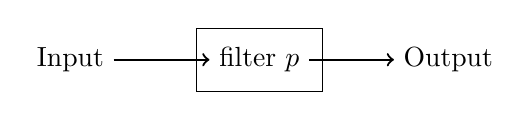
\begin{tikzpicture}[scale=0.8]
      \draw (2, 0) rectangle (4, 1) node (filter) [pos=.5] {filter $p$};
      \draw (0, .5) node (in) {Input}
            (6, .5) node (out) {Output};
      \draw[thick, ->] (in) edge (filter)
                       (filter) edge (out);
      \end{tikzpicture} \\
   \caption{Input: $[x_1, x_2, ..., x_n]$, Output: $[x_1', x_2', ..., x_m']$. and $\forall x_i' \Rightarrow p(x_i')$.}
   \label{fig:filter}
\end{figure}

We can define it in ZF expression:

\be
filter(p, X) = [x_i | x_i \in X, p(x_i)]
\ee

Different from $find$, when there is no element satisfies the predicate, $filter$ returns the empty list. It scans to examine every element one by one:

\be
\begin{array}{rcl}
filter(p,\ [\ ]) & = & [\ ] \\
filter(p,\ x:xs) & = & \begin{cases}
  p(x): & x : filter(p, xs) \\
  otherwise: & filter(p, xs) \\
  \end{cases}
\end{array}
\ee

This definition builds the result from right to left. For iterative implementation, if build the result with $append$, it will degrade to $O(n^2)$.

\begin{algorithmic}[1]
\Function{Filter}{$p, L$}
  \State $L' \gets$ NIL
  \While{$L \neq$ NIL}
    \If{$p$(\Call{First}{$L$})}
      \State $L' \gets$ \textproc{Append}($L'$, \Call{First}{$L$}) \Comment{Linear time}
    \EndIf
    \State $L \gets$ \Call{Rest}{$L$}
  \EndWhile
\EndFunction
\end{algorithmic}

The right way is to use $cons$ instead, however, it builds the result in the reversed order. We can further reverse it within linear time (see the exercise). The nature to build result from right indicates that we can define filter in $foldr$. We need define a function $f$ to test an element against the predicate, if OK, prepend to the result:

\be
f(x, A) = \begin{cases}
  p(x): & x : A \\
  otherwise: & A \\
  \end{cases}
\ee

We also need pass the predicate $p$ to $f$. There are actually 3 parameters as $f(p, x, A)$. Filter is defined in $foldr$ with a Curried form of $f$:

\be
filter(p) = foldr((x, A) \mapsto f(p, x, A), [\ ])
\ee

We can further simplify it (called $\eta$-conversion\cite{slpj-book-1987}) as:

\be
filter(p) = foldr(f(p), [\ ])
\ee

Filter is also a generic concept not only limit to list. We can apply a predicate on any traversable structures to extract the result.

\subsection{Match}
\index{List!matching} \index{List!prefix}
\index{List!suffix} \index{List!infix}

Match is to find a pattern among some structure. Even if we limit to list and string, there are still too many things to cover. We have dedicated chapters about string matching. This section deals with the problem, that given a list $A$, and test if it exits in another list $B$. There are two special cases: to test if $A$ is prefix or suffix of $B$. The $span$ algorithm in (\ref{eq:span}) actually finds a prefix under a certain condition. We can do similar things: to compare each element between $A$ and $B$ from left till meet any different one or reach the end of either list. Define $A \subseteq B$ if $A$ is prefix of $B$:

\be
\begin{array}{rcl}
[\ ] \subseteq B & = & True \\
(a:as) \subseteq [\ ] & = & False \\
(a:as) \subseteq (b:bs) & = & \begin{cases}
  a \neq b: & False \\
  a = b: & as \subseteq bs \\
  \end{cases}
\end{array}
\ee

Prefix testing takes linear time as it scans the lists. However, we can not do suffix testing in this way because it is hard to start from the aligned right ends, and scan backwards for lists. This is different from array. Alternatively, we can reverse both lists in linear time, hence change the problem to prefix testing:

\be
A \supseteq B = reverse(A) \subseteq reverse(B)
\ee

With $\subseteq$ defined, we can test if a list is the sub-list of another one. We call it infix testing. The idea is to scan the target list, and repeatedly applying the prefix testing:

\be
\begin{array}{rcl}
infix?(a:as,\ [\ ]) & = & False \\
infix?(A,\ B) & = & \begin{cases}
  A \subseteq B: & True \\
  otherwise: & infix?(A, B') \\
  \end{cases}
\end{array}
\ee

For the edge case that $A$ is empty, we define empty is infix of any list. Because $[\ ] \subseteq B$ is always true, it gives the right result. It also evaluates $infix?([\ ], [\ ])$ correctly. Below is the corresponding iterative implementation:

\begin{algorithmic}[1]
\Function{Is-Infix}{$A, B$}
  \If{$A = $ NIL}
    \State \Return TRUE
  \EndIf
  \State $n \gets |A|$
  \While{$B \neq$ NIL and $n \leq |B|$}
    \If{$A \subseteq B$}
      \State \Return TRUE
    \EndIf
    \State $B \gets$ \Call{Rest}{$B$}
  \EndWhile
  \State \Return FALSE
\EndFunction
\end{algorithmic}

Because prefix testing runs in linear time, and it is called in the loop of scan. This algorithm is bound to $O(nm)$, where $m, n$ are the length of the two lists respectively. It is an interesting problem to improve this `position by position' scan algorithm to linear time, even when we apply it to arrays. Chapter 13 introduces some smart methods, like the Knuth-Morris-Pratt (KMP) algorithm and Boyer-Moore algorithm. Appendix C introduces another method called suffix-tree.

In a symmetric way, we can enumerate all suffixes of $B$, and check if $A$ is prefix of any of them:

\be
infix?(A, B) = \exists S \in \textit{suffixes}(B), A \subseteq S
\ee

This can be implemented with list comprehension as below example Haskell program:

\begin{Haskell}
isInfixOf a b = (not . null) [ s | s <- tails(b), a `isPrefixOf` s]
\end{Haskell}

Where function \texttt{isPrefixOf} does the prefixing testing, \texttt{tails} generates all suffixes of a given list. We left its implementation as an exercise.

\begin{Exercise}
\Question{Implement the linear time existence testing algorithm.}
\Question{Implement the iterative look up algorithm.}
\Question{Implement the linear time filter algorithm through $reverse$.}
\Question{Implement the iterative prefix testing algorithm.}
\Question{Implement the algorithm to enumerate all suffixes of a list.}
\end{Exercise}

\section{zip and unzip}
\index{List!zip} \index{List!unzip}

The assoc list of paired values is often used as a light weighted dictionary for small set of data. It is easier to build assoc list than tree or heap based dictionary, although the look up performance of assoc list is linear instead of logarithm. In the `$n$-lights' puzzle, we build the assoc list as below:

\[
map(i \mapsto (i, 0),\ [1, 2, ..., n])
\]

More often, we need 'zip' two lists to one. We can define a $zip$ function to do that:

\be
\begin{array}{rcl}
zip(A,\ [\ ]) & = & [\ ] \\
zip([\ ],\ B) & = & [\ ] \\
zip(a:as,\ b:bs) & = & (a, b) : zip(as, bs) \\
\end{array}
\ee

This algorithm works even the two lists have different length. The result length equals to the shorter one. We can even use it to zip infinite lists (under lazy evaluation if both are infinite), for example\footnote{In Haskell: \texttt{zip (repeat 0) [1..n]}}:

\[
zip([0, 0, ...], [1, 2, ..., n])
\]

For a list of words, we can index them with numbers as:

\[
zip([1, 2, ...], [a, an, another, ...])
\]

$zip$ build the result from right. We can also define it with $foldr$. It is bound to $O(m)$ time, where $m$ is the length of the shorter list. When implement the iterative $zip$, the performance will drop to quadratic if using $append$, unless with the reference to the tail position.

\begin{algorithmic}[1]
\Function{Zip}{$A, B$}
  \State $C \gets$ NIL
  \While{$A \neq$ NIL and $B \neq$ NIL}
    \State $C \gets $ \textproc{Append}(C, (\Call{First}{$A$}, \Call{First}{$B$})) \Comment{Linear time}
    \State $A \gets$ \Call{Rest}{$A$}
    \State $B \gets$ \Call{Rest}{$B$}
  \EndWhile
  \State \Return $C$
\EndFunction
\end{algorithmic}

To avoid $append$, we can use 'cons' then reverse the result. However, it can not deal with two infinite lists. In imperative settings, we can also re-use $A$ to store the result (treat it as transform a list of elements to a list of pairs).

We can extend to $zip$ multiple lists to one. Some programming libraries provide, \texttt{zip}, \texttt{zip3}, \texttt{zip4}, ..., till \texttt{zip7}. Sometimes, we don't want to build a list of pairs, but apply a combinator function. For example, given a list of unit prices $[1.00, 0.80, 10.05, ...]$ for fruits: apple, orange, banana, ... When customer has a list of quantities, like $[3, 1, 0, ...]$, means this customer, buys 3 apples, 1 orange, 0 banana, ... Below program generates a payment list:

\[
\begin{array}{rcl}
pays(U,\ [\ ]) & = & [\ ] \\
pays([\ ],\ Q) & = & [\ ] \\
pays(u:us,\ q:qs) & = & (u \cdot q) : pays(us, qs) \\
\end{array}
\]

It is same as the $zip$ function except uses multiply but not 'cons' to combine elements. We can abstract the combinator as a function $f$, and pass it to $zip$ to build a generic algorithm:

\be
\begin{array}{rcl}
zipWith(f, A,\ [\ ]) & = & [\ ] \\
zipWith(f, [\ ],\ B) & = & [\ ] \\
zipWith(f, a:as,\ b:bs) & = & f(a, b) : zipWith(f, as, bs) \\
\end{array}
\ee

Here is an example that defines the inner-product (or dot-product)\cite{wiki-dot-product} through $zipWith$:

\be
A \cdot B = sum(zipWith(\cdot, A, B))
\ee

$unzip$ is the inverse operation of $zip$. It converts a list of pairs to two separated lists. Below is its definition with $foldr$ in Curried form:

\be
unzip = foldr((a, b), (A, B) \mapsto (a : A, b : B), ([\ ], [\ ]))
\ee

We fold from a pair of empty lists, break $a, b$ from the pairs and prepend them to the two intermediate lists respectively. We can also use $fst$ and $snd$ explicitly as:

\[
(p, P) \mapsto (fst(p) : fst(P), snd(p) : snd(P))
\]

For the fruits example, suppose the unit price is stored in a assoc list: $U = [(apple, 1.00), (orange, 0.80), (banana, 10.05), ...]$ for lookup, for example $lookup(melon, U)$. The purchase quantity is a assoc list: $Q = [(apple, 3), (orange, 1), (banana, 0), ...]$. How to calculate the total payment? The straight forward way is to extract the unit price and the quantity lists, then compute their inner-product:

\be
pay = sum(zipWith(\cdot, snd(unzip(U)), snd(unzip(Q))))
\ee

As an example, let's see how to use $zipWith$ to define infinite Fibonacci numbers with lazy evaluation:

\be
F = 0 : 1 : zipWith(+, F, F')
\ee

Where $F$ is the infinite list of Fibonacci numbers, starts from 0 and 1. $F'$ is the rest Fibonacci numbers without the first one. From the third, every Fibonacci number is the sum of numbers from $F$ and $F'$ at the same position. Below example program list the first 15 Fibonacci numbers:

\begin{Haskell}
fib = 0 : 1 : zipWith (+) fib (tail fib)

take 15 fib
[0,1,1,2,3,5,8,13,21,34,55,89,144,233,377]
\end{Haskell}

$zip$ and $unzip$ are generic. We can expand to $zip$ two trees, where the nodes contain paired elements from both. When traverse a collection of elements, we can also use the generic $zip$ and $unzip$ to track the path, this is a method to mimic the `parent' reference in imperative implementation (last chapter of \cite{learn-haskell}).

\begin{Exercise}
\Question{Design the iota ($I$) algorithm for below usages:
  \begin{itemize}
  \item $iota(..., n) = [1, 2, 3, ..., n]$;
  \item $iota(m, n) = [m, m + 1, m + 2, ..., n]$, where $m \leq n$;
  \item $iota(m, m+a, ..., n) = [m, m + a, m + 2a, ..., n]$;
  \item $iota(m, m, ...) = repeat(m) = [m, m, m, ...]$;
  \item $iota(m, ...) = [m, m + 1, m + 2, ... ]$.
  \end{itemize}
  The last two cases are about infinite list. One possible implementation is through streaming and lazy evaluation (\cite{SICP} and \cite{learn-haskell}).}

\Question{Implement the linear time imperative $zip$ algorithm}

\Question{Define $zip$ with $foldr$.}

\Question{For the fruits example, suppose the quantity assoc list only contains the items with none-zero quantity. i.e. instead of
\[
Q = [(apple, 3), (banana, 0), (orange, 1), ...]
\]
but
\[
Q = [(apple, 3), (orange, 1), ...]
\]
because customer does not buy banana. Design a program to calculate the total payment.}

\Question{Implement $lastAt$ with $zip$.}

\end{Exercise}

\section{Further reading}
List is the fundamental thing to build more complex data structures and algorithms particularly in functional settings. We introduced elementary algorithms to construct, access, update, and transform list; how to search, filter data, and compute atop list. Although most programming environments provide pre-defined tools and libraries to support list, we should not simply treat them as black-boxes. Rabhi and Lapalme introduce many functional algorithms about list in \cite{algo-fp}. Haskell library provides detailed documentation about basic list algorithms. There are materials provide good examples of folding, especially in \cite{fp-pearls}. It also introduces about the {\em fold fusion law}.

\begin{Exercise}

\Question{Design algorithm to remove the duplicated elements in a list. For imperative implementation, the elements should be removed in-place. The original element order should be maintained. What is the complexity of this algorithm? How to simplify it with additional data structure?}

\Question{List can represent decimal non-negative integer. For example 1024 as list is $4 \rightarrow 2 \rightarrow 0 \rightarrow 1$. Generally, $n = d_m...d_2d_1$ can be represented as
$d_1 \rightarrow d_2 \rightarrow ... \rightarrow d_m$. Given two numbers $a$, $b$ in list form. Realize arithmetic operations such as add and subtraction.}

\Question{In imperative settings, a circular linked-list is corrupted, that some node points back to previous one, as shown in figure \ref{fig:circular-list}. When traverse, it falls into infinite loops. Design an algorithm to detect if a list is circular. On top of that, improve it to find the node where loop starts (the node being pointed by two precedents).}

\end{Exercise}

\begin{figure}[htbp]
\centering
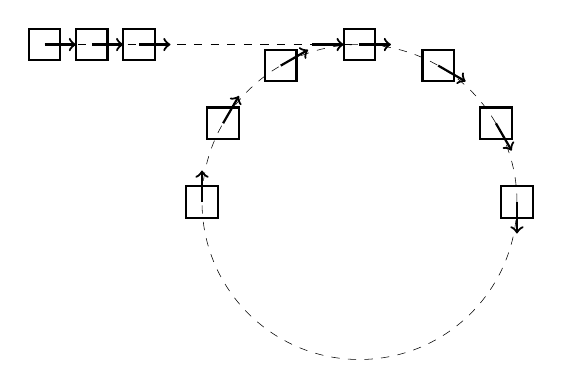
\begin{tikzpicture}[scale=2]
  % trace
  \draw[dashed, very thin] (-2cm, 1cm) -- (0, 1cm);
  \draw[dashed, very thin] (0,0) circle [radius=1cm];

  % leading nodes
  \foreach \x in {-2, -1.7, ..., -1.4} {
    \draw[thick] (\x cm, 1cm) +(-0.1, -0.1) rectangle ++(0.1, 0.1);
    \draw[thick, ->] (\x cm, 1cm) -- +(0.2, 0);
  }

  % cricular starting points
  \draw[thick, ->] (-0.3cm, 1cm) -- (-0.1cm, 1cm);

  % circular nodes
  \foreach \deg/\rot in {90/0, 60/-30, 30/-60, 0/-90, 180/90, 150/60, 120/30} {
    \draw[thick] (\deg : 1cm) +(-0.1, -0.1) rectangle ++(0.1, 0.1);
    \draw[thick, ->] (\deg : 1cm) -- +(\rot : 0.2);
  }
\end{tikzpicture}
\caption{A circular linked-list}
\label{fig:circular-list}
\end{figure}

\ifx\wholebook\relax \else
\begin{thebibliography}{99}

\bibitem{fp-pearls}
Richard Bird. ``Pearls of Functional Algorithm Design''. Cambridge University Press; 1 edition (November 1, 2010). ISBN: 978-0521513388

\bibitem{slpj-book-1987}
Simon L. Peyton Jones. ``The Implementation of Functional Programming Languages''. Prentice-Hall International Series in Computer Since. Prentice Hall (May 1987). ISBN: 978-0134533339

\bibitem{moderncxx}
Andrei Alexandrescu. ``Modern C++ design: Generic Programming and Design Patterns Applied''. Addison Wesley February 01, 2001, ISBN 0-201-70431-5

\bibitem{mittype}
Benjamin C. Pierce. ``Types and Programming Languages''. The MIT Press, 2002. ISBN:0262162091

\bibitem{unplugged}
Xinyu LIU. ``Isomorphism -- mathematics of programming''. 2020. \url{https://github.com/liuxinyu95/unplugged}

\bibitem{SICP}
Harold Abelson, Gerald Jay Sussman, Julie Sussman. ``Structure and Interpretation of Computer Programs, 2nd Edition''. MIT Press, 1996, ISBN 0-262-51087-1

\bibitem{okasaki-book}
Chris Okasaki. ``Purely Functional Data Structures''. Cambridge university press, (July 1, 1999), ISBN-13: 978-0521663502

\bibitem{algo-fp}
Fethi Rabhi, Guy Lapalme. ``Algorithms: a functional programming approach''. Second edition. Addison-Wesley, 1999. ISBN: 0201-59604-0

\bibitem{learn-haskell}
Miran Lipovaca. ``Learn You a Haskell for Great Good! A Beginner's Guide''. No Starch Press; 1 edition April 2011, 400 pp. ISBN: 978-1-59327-283-8

\bibitem{erlang}
Joe Armstrong. ``Programming Erlang: Software for a Concurrent World''. Pragmatic Bookshelf; 1 edition (July 18, 2007). ISBN-13: 978-1934356005

\bibitem{wiki-tail-call}
Wikipedia. ``Tail call''. \url{https://en.wikipedia.org/wiki/Tail_call}

\bibitem{sgi-stl-transform}
SGI. ``transform''. \url{http://www.sgi.com/tech/stl/transform.html}

\bibitem{poj-drunk-jailer}
ACM/ICPC. ``The drunk jailer.'' Peking University judge online for ACM/ICPC. \url{http://poj.org/problem?id=1218}.

\bibitem{Haskell-wiki}
Haskell wiki. ``Haskell programming tips''. 4.4 Choose the appropriate fold. \url{http://www.haskell.org/haskellwiki/Haskell_programming_tips}

\bibitem{wiki-dot-product}
Wikipedia. ``Dot product''. \url{https://en.wikipedia.org/wiki/Dot_product}

\end{thebibliography}

\expandafter\enddocument
\fi
